
%% Template by Michal Forisek


\documentclass[a4paper]{report}
\usepackage{slovak}
\usepackage[utf8]{inputenc}
\usepackage{a4wide}
\usepackage{tabularx}
\usepackage{amsfonts}
\usepackage{amssymb}
\usepackage{epsfig}
\usepackage{color}
\usepackage{mathrsfs}
\usepackage{verbatim}
\usepackage{hyperref}


\def\todo#1{[{\color{red} TODO:} {\bf  #1}]}
\def\fixme#1{[{\color{red} FIXME:} {\bf  #1}]}
\def\verify#1{\todo{verify: #1}}

\renewcommand{\implies}{\rightarrow}
\newcommand{\notmodels}{\nvDash}
\newcommand{\union}{\cup}
\newcommand{\provable}{\vdash}
\newcommand{\unprovable}{\nvdash}

\def\noheader{\relax}

\newtheorem{definicia}{Definícia}[section]
\newtheorem{HLPpriklad}{Príklad}[section]
\newenvironment{priklad}[1][]{
    \ifthenelse{\equal{#1}{}}{
        \begin{HLPpriklad}
    }{
        \begin{HLPpriklad}[#1]
    }
    \rm}{\end{HLPpriklad}
}
\newtheorem{veta}{Veta}[section]
\newtheorem{lema}{Lema}[section]


\newenvironment{dokaz}{\trivlist
  \item[\hskip \labelsep{\bfseries Dôkaz:}]}{\endtrivlist}


\begin{document}

\thispagestyle{empty}
\begin{minipage}{0.25\textwidth}
\includegraphics[width=0.9\textwidth]{img/komlogo-new}
\end{minipage}
\begin{minipage}{0.69\textwidth}
\begin{center}
\sc Katedra Informatiky \\
Fakulta Matematiky, Fyziky a Informatiky \\
Univerzita Komenského, Bratislava
\end{center}
\end{minipage}

\vfill
\begin{center}
\begin{minipage}{0.8\textwidth}
\hrule
\bigskip\bigskip
\centerline{\LARGE\sc Krypto II}
\smallskip
\centerline{(spísané poznámky, draft)}
\bigskip
\bigskip
\centerline{\large\sc Vladimír Boža, Peter Perešíni}
\bigskip
\centerline{\large\sc (prednášal RNDr. Martin Stanek, PhD.)}
\bigskip\bigskip
\hrule
\end{minipage}
\end{center}
\vfill
{~}
\hfill verzia zo dňa {\bf\today} 
\eject % EOP i

\section*{Úvod a disclaimer}

Tieto poznámky obsahujú študijné materiály k predmetu 
\emph{Kryptológia II}
na Fakulte matematiky, fyziky a informatiky UK.
Základná verzia bola spísaná podľa prednášky RNDr. Martina Staneka v
roku 2010. Poznámky však nie sú oficiálny študijný materiál, preto
autori neručia za ich aktuálnosť a vhodnosť na štúdium. Navyše, obsah
prednášky sa môže z roka na rok meniť, a preto je odporúčané dávať
pozor na prípadné rozdiely a dopísať si časti nepokryté týmito
poznámkami.

Aby sme umožnoli jednoduchšie spravovanie a udržali poznámky dlhšie
aktuálne, rozhodli sme sa verejne publikovať zdrojové kódy na stránke
\url{http://code.google.com/p/krypto2}. Ak máte akékoľvek pripomienky,
návrhy, opravy, môžete nám ich prostredníctvom tejto stránky oznámiť.

PPershing a U\$ama.


\tableofcontents

\chapter{Úvod}
\label{chapter:uvod}
\section{Prerekvizity a označenia}

\todo{odkaz na skripta z krypto I}

V zvyšnom texte budeme dodržiavať (až na občasné výnimky) nasledujúce
označenia:
\begin{itemize}
\item $A,B$ - účastníci komunikácie, $E$ - útočník, $E(A)$ - útočník
            tváriaci sa ako účastník $A$.
\item $E(p,k), E_k(p)$ - zašifrovanie otvoreného textu $p$ pomocou kľúča $k$
\item $D(c,k), D_k(c)$ - odšifrovanie šifrového textu $c$ pomocou kľúča $k$
\item $E_A(m)$ - zašifrovanie správy $m$ pomocou verejného kľúča účastníka $A$
\item $D_A(c)$ - odšifrovanie správy $c$ pomocou súkromného kľúča účastníka $A$
\item $H(t)$ - spracovanie textu $t$ pomocou hashovacej funkcie $H$
\item $x \inr M$ - $x$ je \emph{náhodne zvolený} prvok množiny $M$
\item $\exists !$ - existuje práve jeden
\item $p(A)$ - pravdepodobnosť javu $A$
\item $p(A|B)$ - podmienená pravdepodobnosť, t.j. aká je pravdepodobnosť javu $A$, ak platí $B$
\end{itemize}

\section{0. prednáška - Ako (ne)šifrovať disky}

V decembri 2009 bola nájdená bezpečnostná chyba v niektorých šifrovaných USB diskoch
(Kingston DataTraveler BlackBox, SanDisk Cruzer Enterprise FIPS Edition a
Verbatim Corporate Secure FIPS Edition). Všetky výrobcovia uvádzajú, že disky
spĺňajú bezpečnostný štandart FIPS 140-2 a používajú úplne rovnaký systém zabezpečenia,
ktorý vyzerá nasledovne:
\begin{itemize}
\item Používateľ zadá disku heslo.
\item Heslo za pretransformuje cez MD5 hash a prvá polovica výslednej hashe sa použije ako kľúč K.
\item Následne sa pomocou AES-256 a kľúča K odšifruje daných 32 bajtov z disku (označme ich $X$). Potom zistí, či
$D_K(X)=C$, kde $C$ je pevne známa konštanta (u všetkých výrobcov dokonca rovnaká). Ak áno, tak sa disk odomkne a dáta sa sprístupnia.
Ak nie, tak sa požiadavka zamietne. Dešifrovanie ostatných dát nezávisí od hesla.
\end{itemize}

\begin{figure}[htp]
    \centering
    \includegraphics[scale=1]{img/00/extern-drive-encryption.1.mps}
    \label{fig:extern_drive_encryption}
    \caption{Šifrovanie externého disku}
\end{figure}

Útok na tento systém je vcelku jednoduchý. Stačí v pamäti prepísať výsledok dešifrovacej transformácie. 

%Viac na:
%\url{http://www.h-online.com/security/news/item/NIST-certified-USB-Flash-drives-with-hardware-encryption-cracked-895308.html}

%A ešte na (pekny dokument nie priamo suvisiaci):
%Investigating 'secure'USB stickspsu.edu [PDF]
%PJ Bakker… - Citeseer
%\url{http://citeseerx.ist.psu.edu/viewdoc/download?doi=10.1.1.84.2539&rep=rep1&type=pdf}



\chapter{Krypto I}
\label{chapter:krypto}
\section{Interaktívne dokazovacie systémy}

V tejto časti sa budeme venovať dokazovacím systémom. Pôjde o akýsi
typ spoločného výpočtu dvoch účastníkov - jedného výpočtovo
neobmedzeného provera $P$ a výpočtovo obmedzeného overovateľa $V$.
Cieľom provera je akýmsi spôsobom presvedčiť overovateľa o znalosti
nejakého faktu.
Formálne,
interaktívnym dokazovacím systémom nazveme dvojicu
$\langle P,V \rangle$, kde $P$ je pravdepodobnostný TS s neobmedzenou výpočtovou silou,
$V$ je pravdepodobnostný TS pracujúci v polynomiálnom čase.
Oba stroje zdieľajú spoločný vstup $x$, môžu počas svojho výpočtu
komunikovať a o akceprovaní resp. zamietaní vstupu $x$ rozhoduje iba
$V$.
IDS pre jazyk $L$ je $\langle P,V \rangle$ pre ktorý platí
\begin{itemize}
\item {\bf úplnosť} - $\forall x \in L: 
    Pr[V\textit{ akceptuje } x \textit{ v systéme } 
        \langle P,V \rangle ] \ge 2/3$
\item {\bf korektnosť} - $\forall P^*: \forall x \not \in L: 
    Pr[V\textit{ akceptuje } x \textit{ v systéme } 
        \langle P^*,V \rangle ] \le 1/3$
\end{itemize}
Prvá podmienka hovorí o tom, že ak $x\in L$, dokazovateľ s veľkou
pravdepodobnosťou presvedčí overovateľa o správnosti.
Naopak, korektnosť tvrdí, že ľubovoľný (podvodný) dokazovateľ
presvedčí overovateľa na zlom vstupe len s nízkou pravdepodobnosťou.

\begin{komentar}
    Pre $L \in P$ je jednoduché navrhnúť IDS. Overovateľ bude ignorovať
    komunikáciu a môže si vypočítať príslušnosť slova sám.
    Pre $L \in NP$ je jednoduché navrhnúť IDS posielajúci práve jednu
    správu - konkrétny dôkaz - výpočet NTS pre problém L.
\end{komentar}

\begin{priklad}
    Uvažujme problém $GNI \not \in NP$ - grafový neizomorfizmus.
    Vstup pozostáva zo zápisu dvoch grafov $G_0, G_1$, akceptovať chceme, keď
    dané dva grafy nie sú izomorfné. Môžeme použiť nasledovný protokol
    pri dôkaze: Uvažujme $k$ kôl, v každom z nich prebehne nasledujúca
    komunikácia:
    \begin{itemize}
        \item $V$ si zvolí $i \inr \{0,1\}$, permutáciu
         $\pi \inr perm(|G_0|)$
        \item $P \send V: H = \pi(G_i)$.
        \item $V \send P: i'$ reprezentujúce graf $G$, s ktorým je $H$
        izomorfný. ($V$ je neobedzene výpočtovo silný)
        \item prover zamietne ak $i \not = i'$.
    \end{itemize}
    Po $k$ úspešných kolách $V$ akceptuje.

    Ak $G_0 \isomorph G_1$, tak $V$ má v každom kole šancu 50\% na
    uhádnutie indexu $i$, pravdepodobnosť akceptovania po $k$ kolách je teda
    $2^{-k}$.
    Naopak, ak $G_0 \not \isomorph G_1$, tak čestný dokazovateľ vie
    vždy odlíšiť indexy a teda akceptujeme s pravdepodobnosťou 1.
\end{priklad}

\todo{dosiahnute vysledky}:
IP = PSPACE
MIP = NEXPTIME


\section{Zero knowledge}
Špeciálnym prípadom interaktívnych dokazovacích systémov sú takzvané
bezznalostné dôkazy. Základná myšlienka sa dá ilustrovať na príklade 
"Alibaba a jaskyňa tajomstiev".

Alibaba na svojich potulkách narazil (alebo skôr naďabil) na jaskyňu,
ktorá sa na vyslovenie čarovnej formuly otvorí. Po dlhšom skúmaní
prišiel na to, že jazkyňa vyzerá ako na obr. \ref{fig:alibaba}. Pretože v
jaskyni neboli žiadne poklady (alebo boli, ale niekto ich stihol
vybrať skorej), Alibaba sa rozhodol zbohatnúť na TV show.
Bude ukazovať, že vie tajnú formulku a nafilmujú ho pritom. Nechce ale
prezradiť tajomstvo zvyšku sveta.

\begin{figure}[htp]
    \centering
    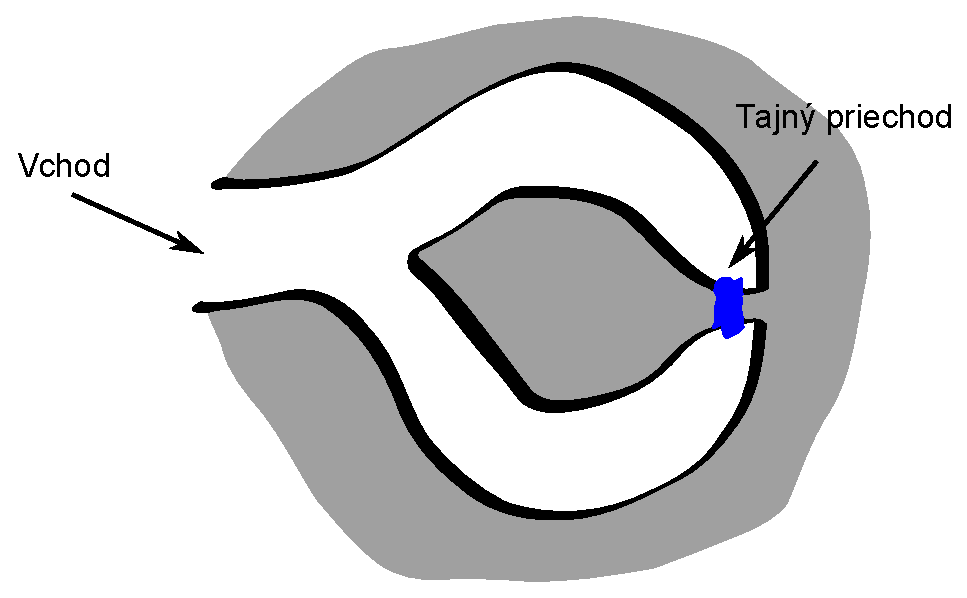
\includegraphics[scale=0.4]{img/x/alibaba}
    
    \label{fig:alibaba}
    \caption{Alibabova jaskyňa}
\end{figure}

Preto sa s filmármi dohodol na nasledujúcom postupe - vôjde do jaskyne
sám. Následne dnu vojde aj filmový štáb a ten zakričí Aladinovi, z
ktorej strany má dôjsť. Ten na demonštráciu znalosti prechádzania cez
steny vyjde zo správnej strany.

Poučenie z príbehu: Môžeme si všimnúť, že Aladin nikomu neprezradí
svoje tajomstvo. Zároveň ale presvedčí štáb o tom, že cez tie steny
chodí, pretože inak by si musel vedieť niekoľkokrát po sebe správne
tipnúť, čo sa mu rozhodnú zakričať, keď dôjdu na rázcestie.
Dôkaz má ale aj ďalšiu vlastnosť - Aladin síce presvedčil štáb, ale
môže presvedčiť aj divákov? Nie. Čo ak bolo napríklad video
"nastrihané" iba na dobré pokusy?

Bezznalostné dokazovacie systémy sú preto také systémy, pri ktorých
dokazovateľ presvedčí overovateľa o svojej pravde bez toho aby mu
prezradil čokoľvek iné. Taktiež, ľubovoľný externý pozorovateľ
komunikácie nemá byť schopný odlíšiť reálny dôkaz od akéhosi
vykonštruovaného.


\todo{zvysok, blackbox simulator}
\todo{ZK pre izomorfizmus}
\todo{preco neizomorfixmus (ako je prezentovany) nie je ZK}
\begin{poznamka}
    Na tomto mieste by sme upozornili čitateľa na fakt, že nami
    prezentovaný algoritmus v predchádzajúcej sekcii na neizomorfizmus grafov
    nie je bezznalostný.
    
    Prečo? Uvažujme falošného verifikátora $V'$,
    ktorý má graf $G$ a vie, že je izomorfný buď s $G_0$ alebo s
    $G_1$. V tomto prípade môže využiť provera $P$ ako orákulum na
    problém izomorfizmu grafov - jednoducho mu pošle $G$, čo je
    validná správa a vráti sa mu index.

    No dobre. A ako súvisí to, že $V'$ vie niečo zistiť s definíciou
    bezznalosti, t.j. s existenciou simulátora? Jednoducho tak, že
    každý polynomiálny simulátor by musel vedieť simulovať komunikáciu
    $P$ s $V'$. Toto ale nemôže vedieť, pretože by sme vedeli v
    polynomiálnom čase riešiť izomorfizmus grafov, čo za predpokladu
    $P\neq NP$ nevieme. Preto dôkaz nie je bezznalostný z definície.
    Záverom teda môžeme usudzovať, že existencia polynomiálneho
    simulátora je naozaj ekvivalentná našej intuícii, čo to znamená
    "bezznalostný".

    Pre záujemcov o bezznalostný algoritmus pre neizomorfizmus grafov
    odporúčame prečítať \cite{nig}, kde je uvedené rozšírenie našeho
    postupu tak, aby $P$ nič neprezradil.
\end{poznamka}

\input{xkrypto1/ot.tex}

\chapter{Krypto II}
\label{chapter:krypto2}
\input{1abs/11abs.tex}

\end{document}
